\documentclass{article}
\usepackage[utf8]{inputenc}
\usepackage[letterpaper]{geometry}
\usepackage{graphicx}
\usepackage{subcaption}
\usepackage{array}
\usepackage{multirow}
\usepackage{amsmath}
\usepackage{hyperref}

\newcommand\MyBox[2]{
  \fbox{\lower0.75cm
    \vbox to 1.7cm{\vfil
      \hbox to 1.7cm{\hfil\parbox{1.4cm}{#1\\#2}\hfil}
      \vfil}%
  }%
}

\title{Association Analysis and Rules Visualization of User Access Patterns from Web Application Logs with R}
\author{Nhon Ai Tran}
\date{\today}

\begin{document}

\maketitle

\section{Results and Discussion}
\subsection{Analysis Using R Statistical Software}
\subsubsection{Association Analysis with "arules" package}
The "arules" package is an interface to C implementation of the association mining algorithm Apriori by Christian Borgelt.  

Of the 17 categories, using the minimum support of 10\%, the categories that site visitors were reading articles mostly frequently are Front Page, On-Air, News, Local, Tech, Sports, and Business.  Articles in other categories such as Weather, MSN-News, Misc., MSN-Sports, Living, Health, Summary, Opinion, and Travel, have less than 10\% hits, with "BBS" being the least visited category with support less than 1\%.

The front page is where the visitors would most likely go first, and the support count for this category reflects this.  But, this might also shows that visitors stayed mostly in the front page section compared to other sections within the site.  Figure \ref{fig:item_frequency} show the relative access frequency for each category. 

\begin{figure}[h!]
  \centering
    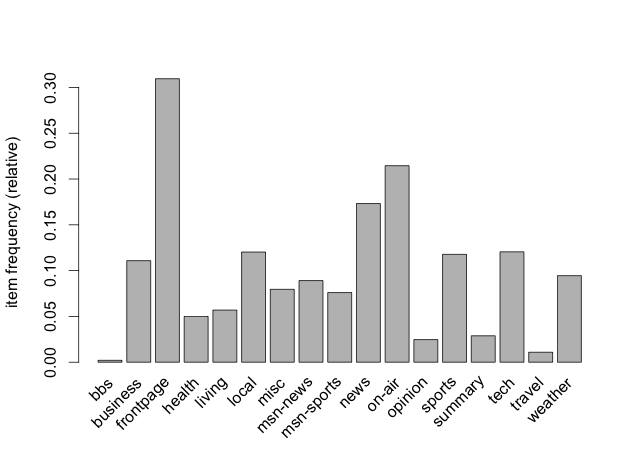
\includegraphics[width=1.0\textwidth]{images/item_frequency_plot}
    \caption{Category access frequency}
    \label{fig:item_frequency}
\end{figure}

The data also shows that 61\% of the visitors read articles from one single category, 31\% read articles from two different categories, and only 8\% ventured out to more than two categories.  Table \ref{tab:ElementLengthDistribution} shows the length distribution per itemset size.  This results explained why there were not many rules with length greater than 3.

\begin{figure}[h!]
  \centering
    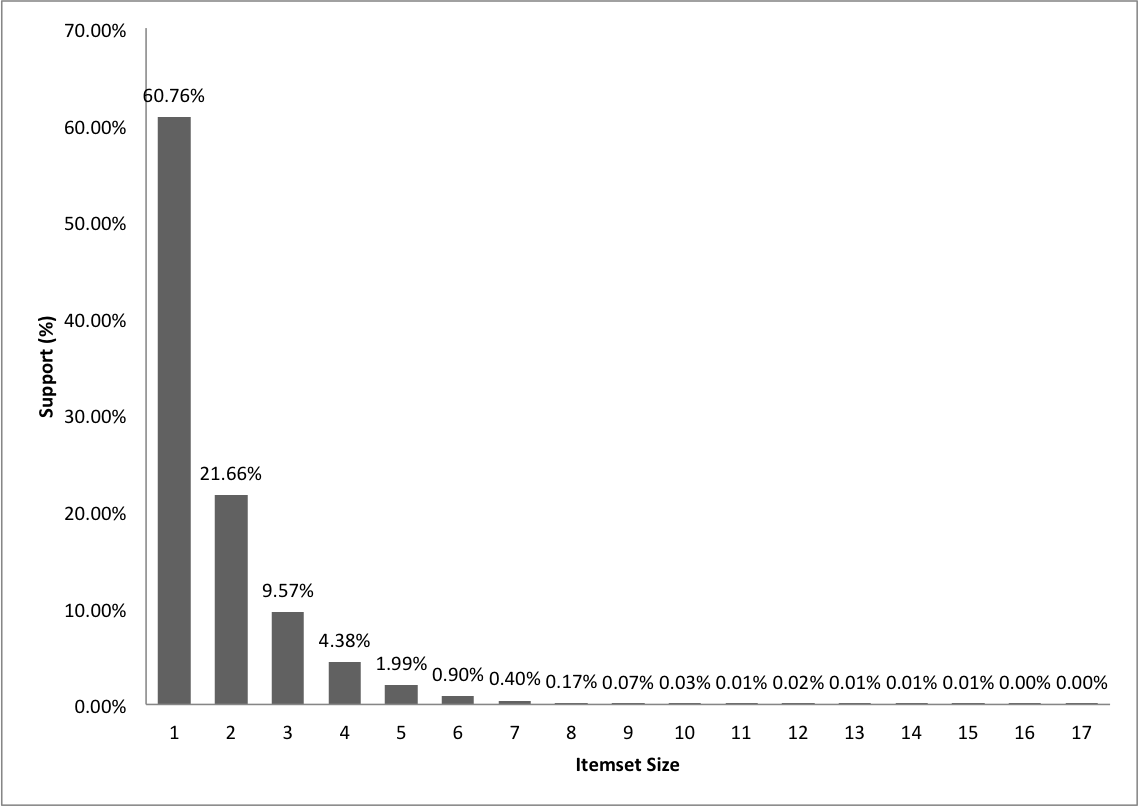
\includegraphics[width=1.0\textwidth]{images/itemset_size_distribution}
    \caption{Itemset size distribution}
    \label{fig:itemset_size_distribution}
\end{figure}

\subsubsection{Rules Visualization with "arulesViz" package}
One of the challenges that data analysts face while mining association rules is the mining process often results in large number of frequent association rules.  This makes the analysis task very time consuming, or worse potentially missing interesting rules due to the high volume of rules that the data analysts must to wade through.  This is where data visualization proves to be very useful in assisting with the analysis tasks.  

For example, for our data set, the top five rules with respect to the support measure ares:
   lhs           rhs              support confidence     lift
1  {misc}     => {on-air}     0.032275760  0.5003742 1.932293
2  {summary}  => {on-air}     0.014723329  0.5057789 1.953164
3  {misc,                                                    
    news}     => {local}      0.005349549  0.5247525 4.346291
4  {misc,                                                    
    weather}  => {local}      0.004593269  0.5725748 4.742382
5  {misc,                                                    
    summary}  => {on-air}     0.004155884  0.8611701 3.325577

Clearly, going through the rules in this tabular format is not a viable option if we are faced with hundreds or thousands rules.  The "arulesViz" visualization package provides many visualization techniques to analyze the extracted association rules graphically.  
\\\\
\textbf{Scatter Plots}\\
Scatter plot is one of the most simple, yet effective graphical method for finding relationship between two interest measures.  The default option is plotting the support and confidence measures.  We also can add the lift measure, which is used as color of the data points.  Figure \ref{fig:interactive} shows the scatter plot of lift and support with confidence as the color of the data points.  From the plot, we can easily see that majority of the rules are in between 1-2\% support, with some rules having high confidence with lift measure greater than 2.  This means these rules are highly correlated.  

Here is where the "interactive" feature, which allows the data analysts to explore the rule interactively, would be most helpful. The analysts can view specific set of rules by using the "inspect" command, filter the set by using "filter" command, or view specific region of the plot as shown in highlighted rectangle by using the "zoom in" command.  This feature is extreme helpful in allowing the data analysts to "slice and dice" the data at different granularity levels.
\begin{figure}[h!]
  \centering
    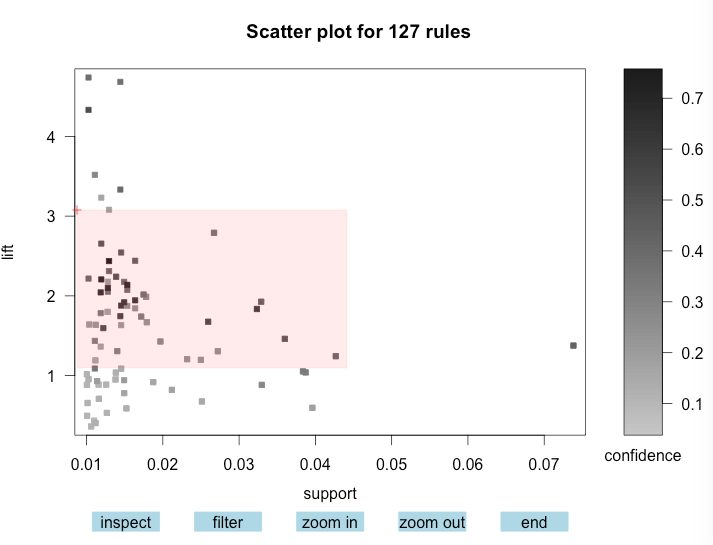
\includegraphics[width=1.0\textwidth]{images/interactive}
    \caption{Analyzing association rules with scatter plot interactively.}
    \label{fig:interactive}
\end{figure}
\\\\
\textbf{Matrix-based Visualization}\\
The matrix-based visualization shows the antecedent and consequent itemsets in matrix format on x-axis and y-axis, respectively.  The lift measure is used as color of the entries in the matrix.   

\begin{figure}[h!]
\begin{subfigure}{.5\textwidth}
  \centering
  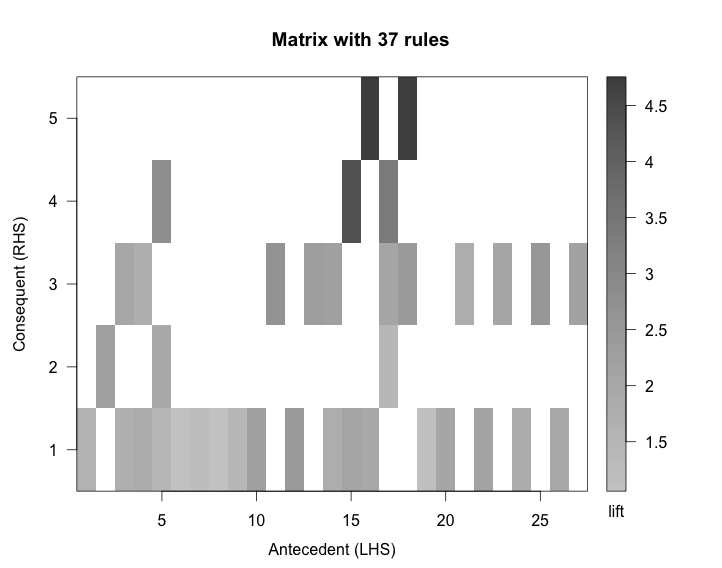
\includegraphics[width=1.1\linewidth]{images/matrix}
  \caption{With lift measure as color}
  \label{fig:matrix}
\end{subfigure}%
\begin{subfigure}{.5\textwidth}
  \centering
  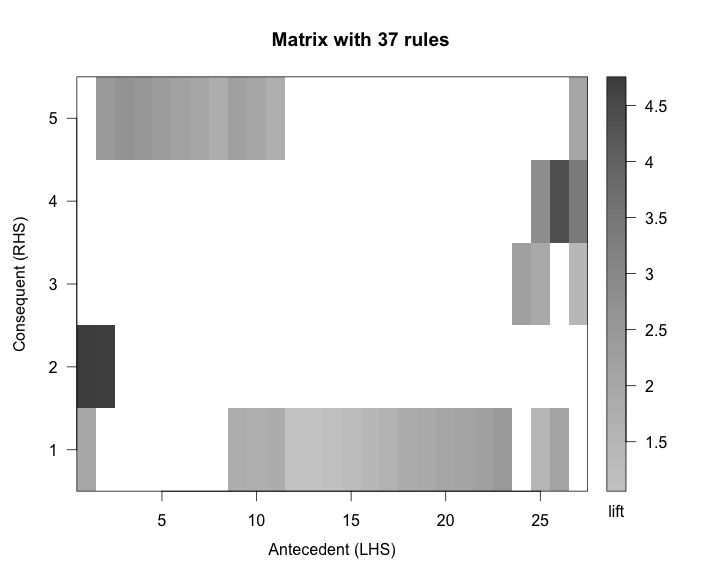
\includegraphics[width=1.1\linewidth]{images/matrix2}
  \caption{Ordering rows and columns to show rules with similar values of lift measures.}
  \label{fig:sorted_matrix}
\end{subfigure}
\caption{Analyzing association rules using matrix-based visualization}
\end{figure}

The rules can also be plot in 3D matrix as shown in Figure \ref{fig:3Dmatrix}
\begin{figure}[h!]
  \centering
    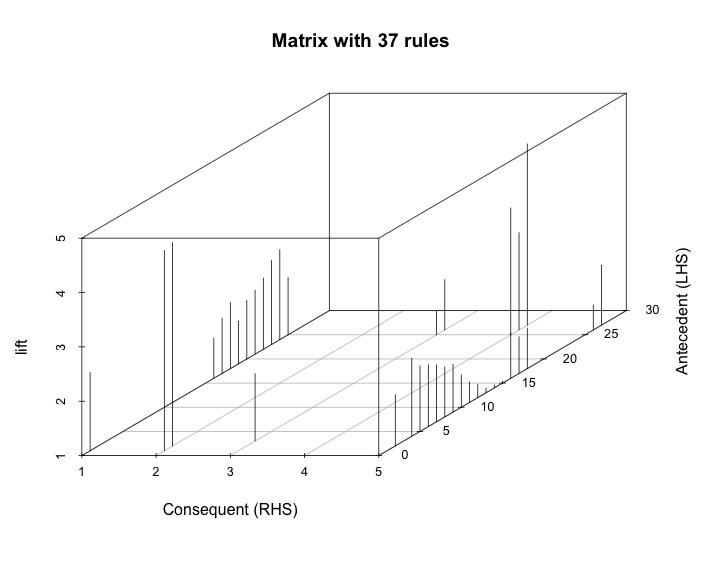
\includegraphics[width=1.0\textwidth]{images/3Dmatrix}
    \caption{Viewing association rules using 3D matrix-based visualization}
    \label{fig:3Dmatrix}
\end{figure}
\\\\
\textbf{Graph Visualization}\\
Graph-based visualization techniques plot the association rules using vertices and edges where the vertices represent itemsets and the edges are the relationship in the rules.  The different shades of the color of the vertices represent the lift measure, darker means stronger correlation, while the size of the vertices represents the support measure with larger balloons mean higher support.  

This technique is the best method to visualize a small set of rules.  It is very intuitive in using directed edges to show the antecedents and consequents of the rules.  However, the plot gets very clutter quickly when the graph becomes to dense with too many rules displayed. Figure \ref{fig:graph} shows an example of the graph-based visualization.
\begin{figure}[h!]
  \centering
    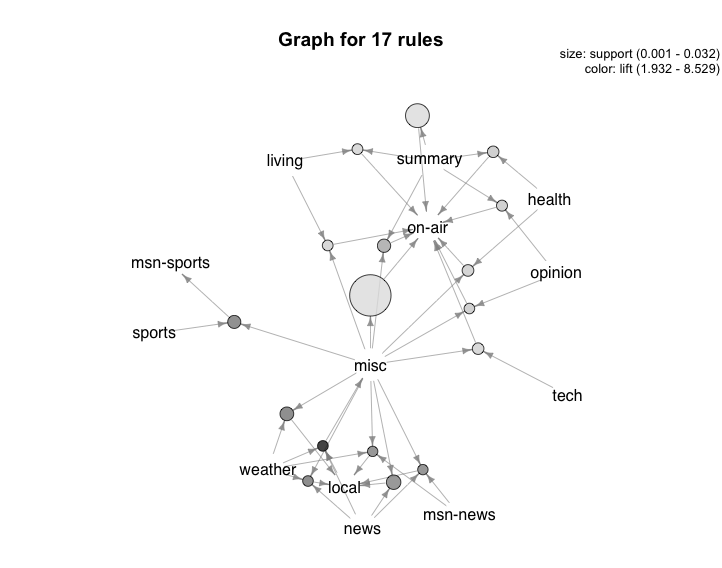
\includegraphics[width=1.0\textwidth]{images/graph}
    \caption{Viewing association rules using graph}
    \label{fig:graph}
\end{figure}
\\\\
\textbf{Grouped Matrix-Based Visualization}\\
This visualization technique allows grouping of rules via cluster.  The color of the balloons represent the aggregated lift measure, while the size of the balloon shows the aggregated support measure.  The number of antecedents and the most frequent items in the group are displayed as the labels the columns.  For example, Figure \ref{fig:grouped} shows the most interesting according to lift measure is the $\{local +2\} \Rightarrow \{misc\}$ rule at the top-left corner.
\begin{figure}[h!]
  \centering
    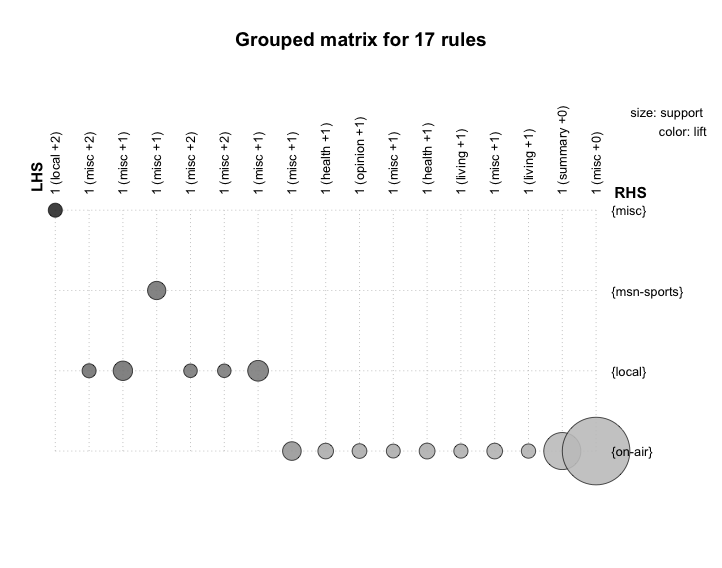
\includegraphics[width=1.0\textwidth]{images/grouped}
    \caption{Viewing association rules using grouped matrix-based visualization}
    \label{fig:grouped}
\end{figure}
\\\\
\textbf{Parallel Coordinates Plot}\\
Parallel coordinates visualization displays the items on y-axis and x-axis shows the position of the items in the rules, starting from left to right where the right most position is normally the consequents.  For example, for an association rule $\{misc, news\} \Rightarrow \{local\}$, the plot puts "misc" in position 1, "news" in position 2, and "local" in position 3.  The width of the arrow represents support of rule, while the intensity of the color represents confidence.  Figure \ref{fig:paracoord} shows an example of the parallel coordinates plot.   
\begin{figure}[h!]
  \centering
    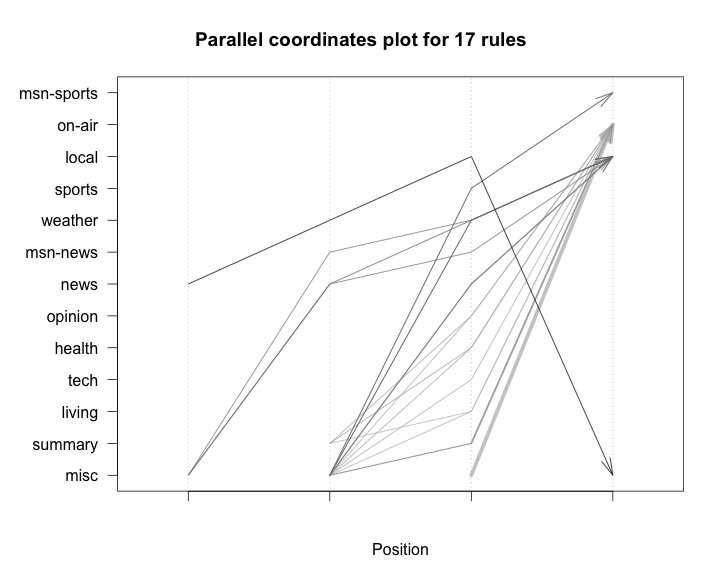
\includegraphics[width=1.0\textwidth]{images/paracoord}
    \caption{Viewing association rules using parallel coordinates plot}
    \label{fig:paracoord}
\end{figure}

\end{document}

